../cictikz/src/cictikz/data/tex/cictikz_preamble.tex

% Mechanical stress components on the channel: F_y vertical, F_x along
% the current direction, F_z along the width.

\definecolor{echarge}{RGB}{30,60,220}
\definecolor{hcharge}{RGB}{220,30,30}
\definecolor{sdgreen}{RGB}{40,150,60}

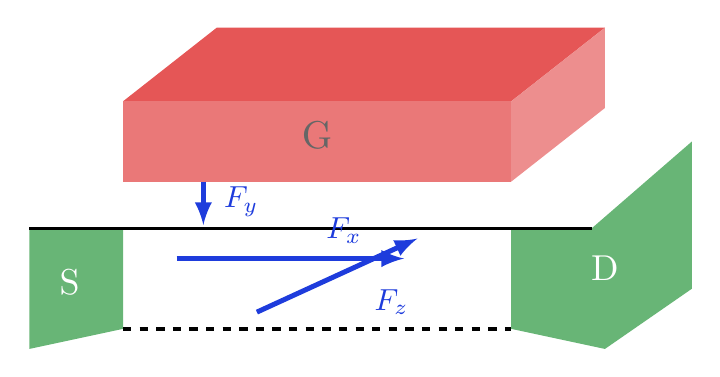
\begin{tikzpicture}[scale=0.85]

  % gate slab, drawn as a shallow 3D box
  \fill[hcharge!75] (1.4,3.4) -- (7.2,3.4) -- (8.6,4.5) -- (2.8,4.5) -- cycle;
  \fill[hcharge!60] (1.4,2.2) rectangle (7.2,3.4);
  \fill[hcharge!50] (7.2,2.2) -- (8.6,3.3) -- (8.6,4.5) -- (7.2,3.4) -- cycle;
  \node[anchor=center, scale=1.4, black!60] at (4.3,2.9) {G};

  % source and drain diffusions
  \fill[sdgreen!70] (0.0,1.5) -- (1.4,1.5) -- (1.4,0.0) -- (0.0,-0.3) -- cycle;
  \fill[sdgreen!70] (7.2,1.5) -- (8.4,1.5) -- (9.9,2.8) -- (9.9,0.6) -- (8.6,-0.3) -- (7.2,0.0) -- cycle;
  \node[anchor=center, scale=1.3, white] at (0.6,0.7) {S};
  \node[anchor=center, scale=1.3, white] at (8.6,0.9) {D};

  % channel surface line
  \draw[line width=1.2pt] (0.0,1.5) -- (8.4,1.5);
  \draw[line width=1.2pt, dashed] (1.4,0.0) -- (7.2,0.0);

  % the three force components
  \draw[echarge, line width=1.8pt, -latex] (2.6,2.2) -- (2.6,1.55);
  \node[echarge, anchor=west, scale=1.1] at (2.75,1.9) {$F_y$};
  \draw[echarge, line width=1.8pt, -latex] (2.2,1.05) -- (5.6,1.05);
  \node[echarge, anchor=south, scale=1.1] at (4.7,1.12) {$F_x$};
  \draw[echarge, line width=1.8pt, -latex] (3.4,0.25) -- (5.8,1.35);
  \node[echarge, anchor=north west, scale=1.1] at (5.0,0.75) {$F_z$};

\end{tikzpicture}
\end{document}
